% Options for packages loaded elsewhere
\PassOptionsToPackage{unicode}{hyperref}
\PassOptionsToPackage{hyphens}{url}
%
\documentclass[
]{article}
\usepackage{amsmath,amssymb}
\usepackage{iftex}
\ifPDFTeX
  \usepackage[T1]{fontenc}
  \usepackage[utf8]{inputenc}
  \usepackage{textcomp} % provide euro and other symbols
\else % if luatex or xetex
  \usepackage{unicode-math} % this also loads fontspec
  \defaultfontfeatures{Scale=MatchLowercase}
  \defaultfontfeatures[\rmfamily]{Ligatures=TeX,Scale=1}
\fi
\usepackage{lmodern}
\ifPDFTeX\else
  % xetex/luatex font selection
\fi
% Use upquote if available, for straight quotes in verbatim environments
\IfFileExists{upquote.sty}{\usepackage{upquote}}{}
\IfFileExists{microtype.sty}{% use microtype if available
  \usepackage[]{microtype}
  \UseMicrotypeSet[protrusion]{basicmath} % disable protrusion for tt fonts
}{}
\makeatletter
\@ifundefined{KOMAClassName}{% if non-KOMA class
  \IfFileExists{parskip.sty}{%
    \usepackage{parskip}
  }{% else
    \setlength{\parindent}{0pt}
    \setlength{\parskip}{6pt plus 2pt minus 1pt}}
}{% if KOMA class
  \KOMAoptions{parskip=half}}
\makeatother
\usepackage{xcolor}
\usepackage[margin=1in]{geometry}
\usepackage{color}
\usepackage{fancyvrb}
\newcommand{\VerbBar}{|}
\newcommand{\VERB}{\Verb[commandchars=\\\{\}]}
\DefineVerbatimEnvironment{Highlighting}{Verbatim}{commandchars=\\\{\}}
% Add ',fontsize=\small' for more characters per line
\usepackage{framed}
\definecolor{shadecolor}{RGB}{248,248,248}
\newenvironment{Shaded}{\begin{snugshade}}{\end{snugshade}}
\newcommand{\AlertTok}[1]{\textcolor[rgb]{0.94,0.16,0.16}{#1}}
\newcommand{\AnnotationTok}[1]{\textcolor[rgb]{0.56,0.35,0.01}{\textbf{\textit{#1}}}}
\newcommand{\AttributeTok}[1]{\textcolor[rgb]{0.13,0.29,0.53}{#1}}
\newcommand{\BaseNTok}[1]{\textcolor[rgb]{0.00,0.00,0.81}{#1}}
\newcommand{\BuiltInTok}[1]{#1}
\newcommand{\CharTok}[1]{\textcolor[rgb]{0.31,0.60,0.02}{#1}}
\newcommand{\CommentTok}[1]{\textcolor[rgb]{0.56,0.35,0.01}{\textit{#1}}}
\newcommand{\CommentVarTok}[1]{\textcolor[rgb]{0.56,0.35,0.01}{\textbf{\textit{#1}}}}
\newcommand{\ConstantTok}[1]{\textcolor[rgb]{0.56,0.35,0.01}{#1}}
\newcommand{\ControlFlowTok}[1]{\textcolor[rgb]{0.13,0.29,0.53}{\textbf{#1}}}
\newcommand{\DataTypeTok}[1]{\textcolor[rgb]{0.13,0.29,0.53}{#1}}
\newcommand{\DecValTok}[1]{\textcolor[rgb]{0.00,0.00,0.81}{#1}}
\newcommand{\DocumentationTok}[1]{\textcolor[rgb]{0.56,0.35,0.01}{\textbf{\textit{#1}}}}
\newcommand{\ErrorTok}[1]{\textcolor[rgb]{0.64,0.00,0.00}{\textbf{#1}}}
\newcommand{\ExtensionTok}[1]{#1}
\newcommand{\FloatTok}[1]{\textcolor[rgb]{0.00,0.00,0.81}{#1}}
\newcommand{\FunctionTok}[1]{\textcolor[rgb]{0.13,0.29,0.53}{\textbf{#1}}}
\newcommand{\ImportTok}[1]{#1}
\newcommand{\InformationTok}[1]{\textcolor[rgb]{0.56,0.35,0.01}{\textbf{\textit{#1}}}}
\newcommand{\KeywordTok}[1]{\textcolor[rgb]{0.13,0.29,0.53}{\textbf{#1}}}
\newcommand{\NormalTok}[1]{#1}
\newcommand{\OperatorTok}[1]{\textcolor[rgb]{0.81,0.36,0.00}{\textbf{#1}}}
\newcommand{\OtherTok}[1]{\textcolor[rgb]{0.56,0.35,0.01}{#1}}
\newcommand{\PreprocessorTok}[1]{\textcolor[rgb]{0.56,0.35,0.01}{\textit{#1}}}
\newcommand{\RegionMarkerTok}[1]{#1}
\newcommand{\SpecialCharTok}[1]{\textcolor[rgb]{0.81,0.36,0.00}{\textbf{#1}}}
\newcommand{\SpecialStringTok}[1]{\textcolor[rgb]{0.31,0.60,0.02}{#1}}
\newcommand{\StringTok}[1]{\textcolor[rgb]{0.31,0.60,0.02}{#1}}
\newcommand{\VariableTok}[1]{\textcolor[rgb]{0.00,0.00,0.00}{#1}}
\newcommand{\VerbatimStringTok}[1]{\textcolor[rgb]{0.31,0.60,0.02}{#1}}
\newcommand{\WarningTok}[1]{\textcolor[rgb]{0.56,0.35,0.01}{\textbf{\textit{#1}}}}
\usepackage{graphicx}
\makeatletter
\def\maxwidth{\ifdim\Gin@nat@width>\linewidth\linewidth\else\Gin@nat@width\fi}
\def\maxheight{\ifdim\Gin@nat@height>\textheight\textheight\else\Gin@nat@height\fi}
\makeatother
% Scale images if necessary, so that they will not overflow the page
% margins by default, and it is still possible to overwrite the defaults
% using explicit options in \includegraphics[width, height, ...]{}
\setkeys{Gin}{width=\maxwidth,height=\maxheight,keepaspectratio}
% Set default figure placement to htbp
\makeatletter
\def\fps@figure{htbp}
\makeatother
\setlength{\emergencystretch}{3em} % prevent overfull lines
\providecommand{\tightlist}{%
  \setlength{\itemsep}{0pt}\setlength{\parskip}{0pt}}
\setcounter{secnumdepth}{-\maxdimen} % remove section numbering
\ifLuaTeX
  \usepackage{selnolig}  % disable illegal ligatures
\fi
\IfFileExists{bookmark.sty}{\usepackage{bookmark}}{\usepackage{hyperref}}
\IfFileExists{xurl.sty}{\usepackage{xurl}}{} % add URL line breaks if available
\urlstyle{same}
\hypersetup{
  pdftitle={BDMI\_mapping},
  hidelinks,
  pdfcreator={LaTeX via pandoc}}

\title{BDMI\_mapping}
\author{}
\date{\vspace{-2.5em}2022-08-25}

\begin{document}
\maketitle

\hypertarget{region-a}{%
\subsection{region A}\label{region-a}}

Read in vcf files (mapped to N17 and W303) - remove one comment line
first so get header.

\begin{verbatim}
## 
## Attaching package: 'dplyr'
\end{verbatim}

\begin{verbatim}
## The following objects are masked from 'package:stats':
## 
##     filter, lag
\end{verbatim}

\begin{verbatim}
## The following objects are masked from 'package:base':
## 
##     intersect, setdiff, setequal, union
\end{verbatim}

Check that it worked

\begin{Shaded}
\begin{Highlighting}[]
\FunctionTok{head}\NormalTok{(AN)}
\end{Highlighting}
\end{Shaded}

\begin{verbatim}
##           V1   V2 V3 V4 V5      V6   V7
## 1 N_17.chr09 5283  .  G  A 1557.10 PASS
## 2 N_17.chr09 5286  .  T  G 6432.63 PASS
## 3 N_17.chr09 5292  .  A  G 6512.63 PASS
## 4 N_17.chr09 5304  .  T  C 6737.63 PASS
## 5 N_17.chr09 5316  .  A  G 6692.63 PASS
## 6 N_17.chr09 5322  .  C  A 6647.63 PASS
##                                                                                                                                        V8
## 1 AC=1;AF=0.167;AN=6;BaseQRankSum=0.688;DP=525;FS=0;MLEAC=1;MLEAF=0.167;MQ=45.09;MQRankSum=-1.578;QD=11.12;ReadPosRankSum=-0.65;SOR=0.703
## 2                                                            AC=3;AF=0.5;AN=6;DP=526;FS=0;MLEAC=4;MLEAF=0.667;MQ=45.01;QD=33.76;SOR=1.006
## 3                                                            AC=3;AF=0.5;AN=6;DP=534;FS=0;MLEAC=4;MLEAF=0.667;MQ=45.04;QD=31.63;SOR=0.987
## 4                                                            AC=3;AF=0.5;AN=6;DP=549;FS=0;MLEAC=4;MLEAF=0.667;MQ=44.82;QD=35.64;SOR=0.927
## 5                                                            AC=3;AF=0.5;AN=6;DP=576;FS=0;MLEAC=4;MLEAF=0.667;MQ=44.66;QD=28.73;SOR=0.881
## 6                                                            AC=3;AF=0.5;AN=6;DP=570;FS=0;MLEAC=4;MLEAF=0.667;MQ=44.52;QD=31.75;SOR=0.806
##               V9                          V10                               V11
## 1 GT:AD:DP:GQ:PL 0/0/0:316,0:316:0:0,0,0,6232 0/0/1:77,63:140:41:1562,0,41,2020
## 2 GT:AD:DP:GQ:PL 0/0/0:318,0:318:0:0,0,0,1653 1/1/1:0,144:144:99:6445,686,253,0
## 3 GT:AD:DP:GQ:PL 0/0/0:325,0:325:0:0,0,0,1595 1/1/1:0,145:145:99:6525,692,255,0
## 4 GT:AD:DP:GQ:PL 0/0/0:335,0:335:0:0,0,0,2034 1/1/1:0,150:150:99:6750,716,264,0
## 5 GT:AD:DP:GQ:PL 0/0/0:363,0:363:0:0,0,0,1892 1/1/1:0,149:149:99:6705,711,262,0
## 6 GT:AD:DP:GQ:PL 0/0/0:358,0:358:0:0,0,0,3525 1/1/1:0,148:148:99:6660,706,261,0
\end{verbatim}

\begin{Shaded}
\begin{Highlighting}[]
\FunctionTok{head}\NormalTok{(AW)}
\end{Highlighting}
\end{Shaded}

\begin{verbatim}
##           V1   V2 V3 V4 V5      V6   V7
## 1 W303.chr09 1729  .  C  T 15104.7 PASS
## 2 W303.chr09 1734  .  T  C 13187.7 PASS
## 3 W303.chr09 1738  .  C  T 13019.7 PASS
## 4 W303.chr09 1792  .  A  G 33180.7 PASS
## 5 W303.chr09 1810  .  G  A 33672.7 PASS
## 6 W303.chr09 1830  .  T  A 31901.7 PASS
##                                                                                                                                              V8
## 1      AC=2;AF=0.333;AN=6;BaseQRankSum=-0.707;DP=2299;FS=0;MLEAC=2;MLEAF=0.333;MQ=58.76;MQRankSum=-6.455;QD=7.17;ReadPosRankSum=0.458;SOR=0.663
## 2   AC=2;AF=0.333;AN=6;BaseQRankSum=-0.548;DP=2253;FS=0.682;MLEAC=2;MLEAF=0.333;MQ=58.78;MQRankSum=-0.557;QD=6.28;ReadPosRankSum=2.21;SOR=0.613
## 3       AC=2;AF=0.333;AN=6;BaseQRankSum=1.61;DP=2273;FS=0.69;MLEAC=2;MLEAF=0.333;MQ=58.77;MQRankSum=-0.442;QD=6.14;ReadPosRankSum=2.8;SOR=0.571
## 4 AC=2;AF=0.333;AN=6;BaseQRankSum=0.206;DP=2192;FS=2.477;MLEAC=2;MLEAF=0.333;MQ=59.52;MQRankSum=-5.104;QD=15.58;ReadPosRankSum=-0.879;SOR=0.712
## 5  AC=2;AF=0.333;AN=6;BaseQRankSum=4.41;DP=2114;FS=1.113;MLEAC=2;MLEAF=0.333;MQ=59.59;MQRankSum=-5.116;QD=16.07;ReadPosRankSum=-0.255;SOR=0.791
## 6   AC=2;AF=0.333;AN=6;BaseQRankSum=0.083;DP=2032;FS=0.53;MLEAC=2;MLEAF=0.333;MQ=59.52;MQRankSum=-5.461;QD=15.94;ReadPosRankSum=0.019;SOR=0.735
##               V9                                     V10
## 1 GT:AD:DP:GQ:PL 0/0/1:840,265:1105:99:9093,0,1731,34715
## 2 GT:AD:DP:GQ:PL 0/0/1:860,245:1105:99:8274,0,1851,35840
## 3 GT:AD:DP:GQ:PL 0/0/1:875,243:1118:99:8157,0,1902,36322
## 4 GT:AD:DP:GQ:PL 0/0/1:588,539:1127:99:19887,0,147,22080
## 5 GT:AD:DP:GQ:PL 0/0/1:581,529:1110:99:20221,0,156,22468
## 6 GT:AD:DP:GQ:PL 0/0/1:554,520:1074:99:19371,0,102,21001
##                                       V11
## 1 0/0/1:813,188:1001:99:6019,0,1882,33976
## 2  0/0/1:834,160:994:99:4921,0,2029,35122
## 3 0/0/1:843,160:1003:99:4870,0,2056,35360
## 4 0/0/1:633,370:1003:99:13301,0,791,24863
## 5  0/0/1:622,363:985:99:13459,0,779,25066
## 6  0/0/1:580,347:927:99:12538,0,703,23001
\end{verbatim}

Rename the columns.\\
Cut down to the range for A:\\
range for A - YIL166C to YIL156W is region, did transformations YIL151C
to YIL169C\\
For N17 - (??) end to 41322\\
For W303 - 24534 to 62140\\
Go a bit outside (1kb on either end).

Only keep the columns I want.\\
Information wanted: chr(omosome), pos(ition), ref (allele), alt(ernate
allele), qual(ity), a1 (sample), a2 (sample)\\

In last two columns, the format is GT:AD:DP:GQ:PL\\
FORMAT=\textless ID=GT,Number=1,Type=String,Description=``Genotype''\textgreater{}\\
FORMAT=\textless ID=AD,Number=R,Type=Integer,Description=``Allelic
depths for the ref and alt alleles in the order listed''\textgreater{}\\
FORMAT=\textless ID=DP,Number=1,Type=Integer,Description=``Approximate
read depth (reads with MQ=255 or with bad mates are
filtered)''\textgreater{}\\
FORMAT=\textless ID=GQ,Number=1,Type=Integer,Description=``Genotype
Quality''\textgreater{}\\
FORMAT=\textless ID=PL,Number=G,Type=Integer,Description=``Normalized,
Phred-scaled likelihoods for genotypes as defined in the VCF
specification''\textgreater{}\\

Split the last column and make new columns out of the ``AD'' section.\\
FORMAT=\textless ID=AD,Number=R,Type=Integer,Description=``Allelic
depths (high-quality bases)''\textgreater{} - ref, alt\\
Save as a1nref, a1nalt, a2nref, a2nalt.\\

Then calculate the frequencies of paradoxus alleles. For AN (mapped to
paradoxus), it's nref/total. For AW (mapped to cerevsiae), it's
nalt/total. Saved as a1reff, a2reff, a1altf, a2altf.\\
\strut \\
Also found coverage of each SNP as nref+nalt. Saved as a1cov, a2cov.\\

Plot outcome of frequencies. Mapped to paradoxus, with a1reff in black,
a2reff in blue.
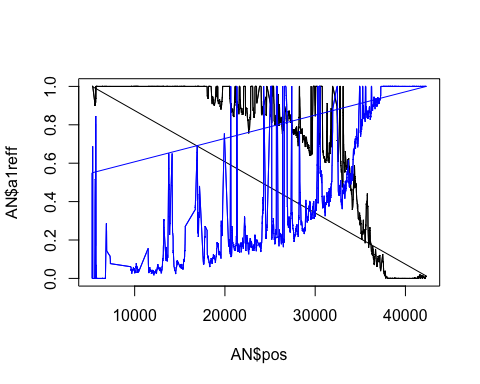
\includegraphics{BDMI_mapping_files/figure-latex/unnamed-chunk-6-1.pdf}

Plot mapped to cerevisiae. a1altf in black, a2altf in blue.
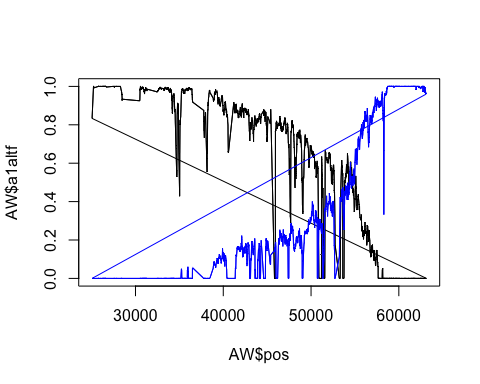
\includegraphics{BDMI_mapping_files/figure-latex/unnamed-chunk-7-1.pdf}

According to Eyal's paper, ``SNPs with excessive depth were removed
because they are suspected as repetitive sequences, using a threshold of
450X total depth across all samples'' (which was two standard deviations
above the mean depth)\\
\strut \\
Find the mean coverage in the region and the SD and make the cutoff 2 SD
above the mean.\\

\begin{Shaded}
\begin{Highlighting}[]
\FunctionTok{mean}\NormalTok{(AN}\SpecialCharTok{$}\NormalTok{a1cov)}
\end{Highlighting}
\end{Shaded}

\begin{verbatim}
## [1] 294.1557
\end{verbatim}

\begin{Shaded}
\begin{Highlighting}[]
\FunctionTok{sd}\NormalTok{(AN}\SpecialCharTok{$}\NormalTok{a1cov)}
\end{Highlighting}
\end{Shaded}

\begin{verbatim}
## [1] 75.40178
\end{verbatim}

\begin{Shaded}
\begin{Highlighting}[]
\NormalTok{cutAN1 }\OtherTok{\textless{}{-}} \FunctionTok{mean}\NormalTok{(AN}\SpecialCharTok{$}\NormalTok{a1cov)}\SpecialCharTok{+}\DecValTok{2}\SpecialCharTok{*}\FunctionTok{sd}\NormalTok{(AN}\SpecialCharTok{$}\NormalTok{a1cov)}

\FunctionTok{mean}\NormalTok{(AN}\SpecialCharTok{$}\NormalTok{a2cov)}
\end{Highlighting}
\end{Shaded}

\begin{verbatim}
## [1] 198.1067
\end{verbatim}

\begin{Shaded}
\begin{Highlighting}[]
\FunctionTok{sd}\NormalTok{(AN}\SpecialCharTok{$}\NormalTok{a2cov)}
\end{Highlighting}
\end{Shaded}

\begin{verbatim}
## [1] 74.56178
\end{verbatim}

\begin{Shaded}
\begin{Highlighting}[]
\NormalTok{cutAN2 }\OtherTok{\textless{}{-}} \FunctionTok{mean}\NormalTok{(AN}\SpecialCharTok{$}\NormalTok{a2cov)}\SpecialCharTok{+}\DecValTok{2}\SpecialCharTok{*}\FunctionTok{sd}\NormalTok{(AN}\SpecialCharTok{$}\NormalTok{a2cov)}

\FunctionTok{mean}\NormalTok{(AW}\SpecialCharTok{$}\NormalTok{a1cov)}
\end{Highlighting}
\end{Shaded}

\begin{verbatim}
## [1] 261.0112
\end{verbatim}

\begin{Shaded}
\begin{Highlighting}[]
\FunctionTok{sd}\NormalTok{(AW}\SpecialCharTok{$}\NormalTok{a1cov)}
\end{Highlighting}
\end{Shaded}

\begin{verbatim}
## [1] 100.5098
\end{verbatim}

\begin{Shaded}
\begin{Highlighting}[]
\NormalTok{cutAW1 }\OtherTok{\textless{}{-}} \FunctionTok{mean}\NormalTok{(AW}\SpecialCharTok{$}\NormalTok{a1cov)}\SpecialCharTok{+}\DecValTok{2}\SpecialCharTok{*}\FunctionTok{sd}\NormalTok{(AW}\SpecialCharTok{$}\NormalTok{a1cov)}

\FunctionTok{mean}\NormalTok{(AW}\SpecialCharTok{$}\NormalTok{a2cov)}
\end{Highlighting}
\end{Shaded}

\begin{verbatim}
## [1] 226.4242
\end{verbatim}

\begin{Shaded}
\begin{Highlighting}[]
\FunctionTok{sd}\NormalTok{(AW}\SpecialCharTok{$}\NormalTok{a2cov)}
\end{Highlighting}
\end{Shaded}

\begin{verbatim}
## [1] 58.0252
\end{verbatim}

\begin{Shaded}
\begin{Highlighting}[]
\NormalTok{cutAW2 }\OtherTok{\textless{}{-}} \FunctionTok{mean}\NormalTok{(AW}\SpecialCharTok{$}\NormalTok{a2cov)}\SpecialCharTok{+}\DecValTok{2}\SpecialCharTok{*}\FunctionTok{sd}\NormalTok{(AW}\SpecialCharTok{$}\NormalTok{a2cov)}
\end{Highlighting}
\end{Shaded}

Now remove outliers in coverage that are higher that 2 SDs above mean.
These may be repetitive sequences. Save as AN/AWcut.

Plot the coverage of the original and versions with cutoff (cutoff in
red and purple).\\
Also add the cutoffs as lines.\\
Also add the frequencies (*400 to fit on plot).

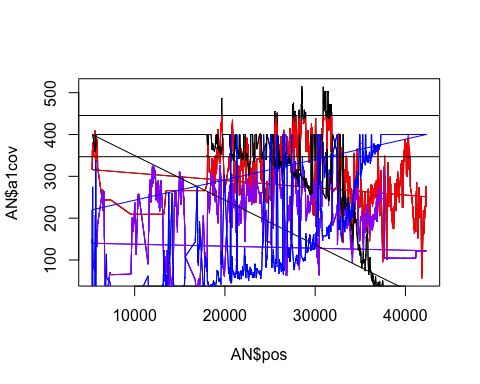
\includegraphics{BDMI_mapping_files/figure-latex/unnamed-chunk-10-1.pdf}
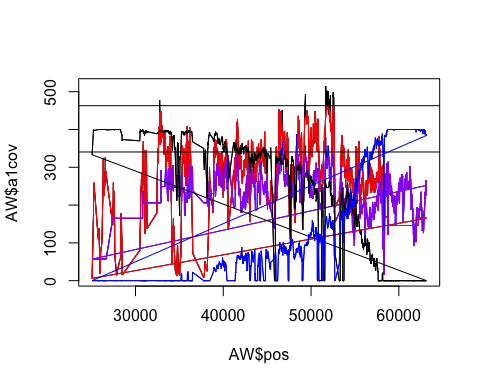
\includegraphics{BDMI_mapping_files/figure-latex/unnamed-chunk-10-2.pdf}
Still not good. Also, large region with very few SNPs in a1.\\
\strut \\
Try cutting off the bottom ones as well as they don't have consistent
coverage.\\
Cutoff is 2 SD below mean.\\
Save as AN/Wcut2.\\
Plot these in green and orange.

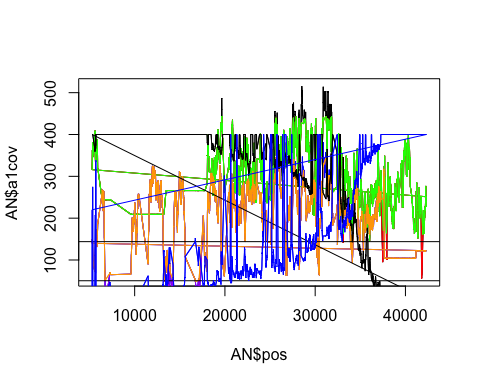
\includegraphics{BDMI_mapping_files/figure-latex/unnamed-chunk-11-1.pdf}
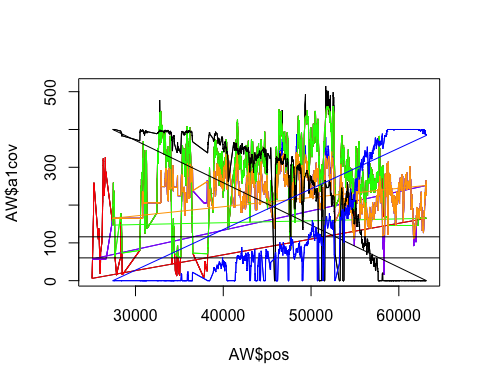
\includegraphics{BDMI_mapping_files/figure-latex/unnamed-chunk-11-2.pdf}
Got rid of some crazy peaks and smoothed it out a bit.\\
\strut \\
Now try requiring that called variants are variable in both samples
(within mapping to a single species).\\
This will cut off the ends, but we're not really interested in those.\\
Then plot again with original (lightest), cut2 (darker) and cut3
(darkest).

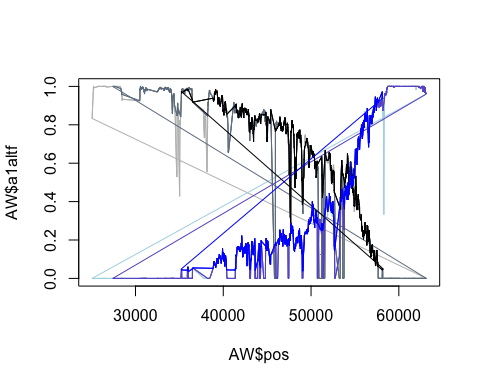
\includegraphics{BDMI_mapping_files/figure-latex/unnamed-chunk-12-1.pdf}
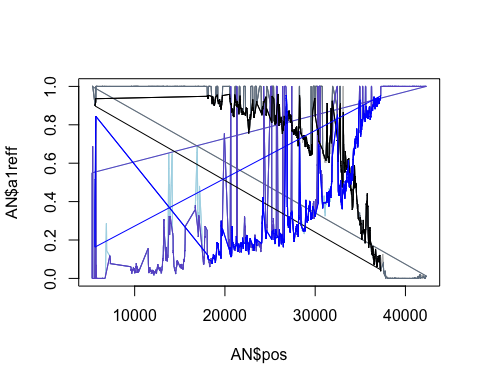
\includegraphics{BDMI_mapping_files/figure-latex/unnamed-chunk-12-2.pdf}
Improved again.\\
Tried requiring certain minimal minor allele frequency but doesn't seem
helpful, almost none with low cutoff.\\
\strut \\
Now will trim SNPs that are quite different from the median around them.
First, need to find out how big the region is.

\begin{Shaded}
\begin{Highlighting}[]
\FunctionTok{min}\NormalTok{(ANcut3}\SpecialCharTok{$}\NormalTok{pos)}
\end{Highlighting}
\end{Shaded}

\begin{verbatim}
## [1] 5601
\end{verbatim}

\begin{Shaded}
\begin{Highlighting}[]
\FunctionTok{max}\NormalTok{(ANcut3}\SpecialCharTok{$}\NormalTok{pos)}
\end{Highlighting}
\end{Shaded}

\begin{verbatim}
## [1] 37264
\end{verbatim}

\begin{Shaded}
\begin{Highlighting}[]
\FunctionTok{min}\NormalTok{(AWcut3}\SpecialCharTok{$}\NormalTok{pos)}
\end{Highlighting}
\end{Shaded}

\begin{verbatim}
## [1] 35236
\end{verbatim}

\begin{Shaded}
\begin{Highlighting}[]
\FunctionTok{max}\NormalTok{(AWcut3}\SpecialCharTok{$}\NormalTok{pos)}
\end{Highlighting}
\end{Shaded}

\begin{verbatim}
## [1] 58160
\end{verbatim}

Based on this, the region in paradoxus (N) is:\\
37273-5601=31672bp long\\
We expect the frequency to go from 0 to 1 in this region so, if went up
consistently, would change by 0.1 within:\\
31672/10=3167.2\\
so should be reasonable to expect that every SNP should be within 0.1 of
the median within \textasciitilde1584bp.\\
\strut \\
For cerevisiae (W): 57641-35236= 22405bc long\\
22405/10 = 2240.5\\
So will use 1120bp.\\
\strut \\
Also, do regions every 100bp. Plots the old frequencies from SNPs in
lighter colours and post-cut in darker colours. First, need to rename
columns.

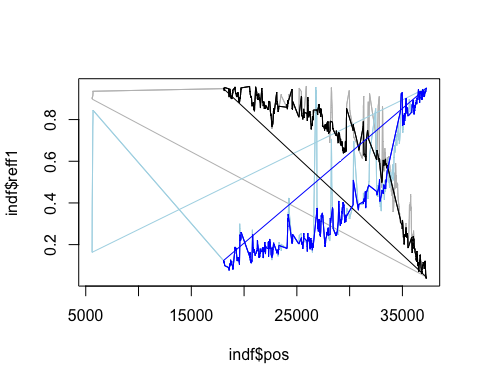
\includegraphics{BDMI_mapping_files/figure-latex/unnamed-chunk-14-1.pdf}
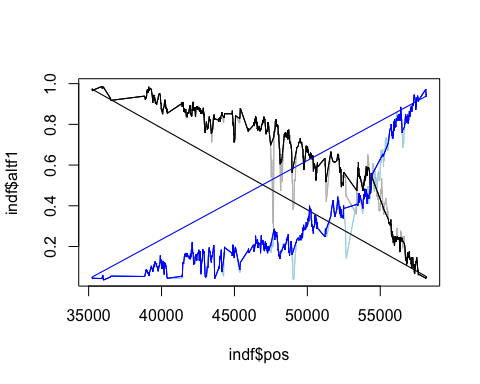
\includegraphics{BDMI_mapping_files/figure-latex/unnamed-chunk-14-2.pdf}

Find out how many cut:

\begin{Shaded}
\begin{Highlighting}[]
\FunctionTok{length}\NormalTok{(ANcut3}\SpecialCharTok{$}\NormalTok{chr)}
\end{Highlighting}
\end{Shaded}

\begin{verbatim}
## [1] 2258
\end{verbatim}

\begin{Shaded}
\begin{Highlighting}[]
\FunctionTok{length}\NormalTok{(ANcut4}\SpecialCharTok{$}\NormalTok{chr)}
\end{Highlighting}
\end{Shaded}

\begin{verbatim}
## [1] 1628
\end{verbatim}

\begin{Shaded}
\begin{Highlighting}[]
\FunctionTok{length}\NormalTok{(AWcut3}\SpecialCharTok{$}\NormalTok{chr)}
\end{Highlighting}
\end{Shaded}

\begin{verbatim}
## [1] 2514
\end{verbatim}

\begin{Shaded}
\begin{Highlighting}[]
\FunctionTok{length}\NormalTok{(AWcut4}\SpecialCharTok{$}\NormalTok{chr)}
\end{Highlighting}
\end{Shaded}

\begin{verbatim}
## [1] 2112
\end{verbatim}

Now plot with loess smoothing. Loess with span=0.25. Do for those mapped
to paradoxus first.
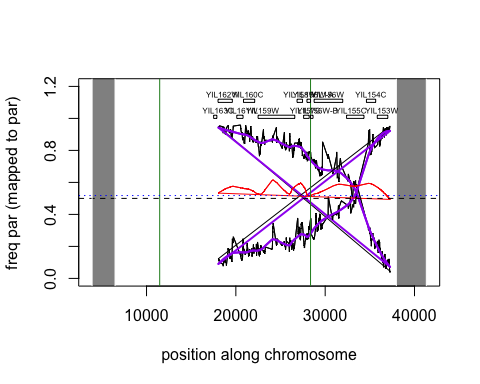
\includegraphics{BDMI_mapping_files/figure-latex/unnamed-chunk-16-1.pdf}
Plot for those mapped to paradoxus (N17) with loess smoothing.\\
Borders of original region in forestgreen. Rectangles where did
transformations.\\
Bottom 5\% of sum of fits in dotted blue line.\\
\strut \\
Now plot with loess smoothing. Loess with span=0.25. Do for those mapped
to cerevisiae.
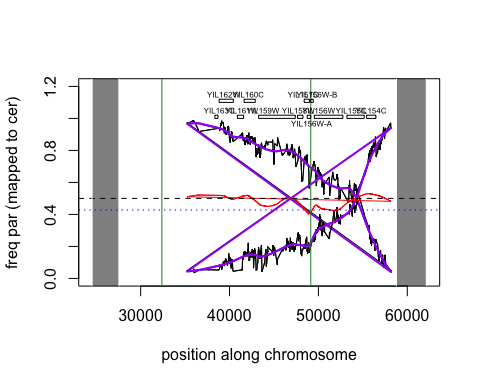
\includegraphics{BDMI_mapping_files/figure-latex/unnamed-chunk-17-1.pdf}
Plot for those mapped to cerevisiae (W303).\\
Borders of original region in forestgreen. Rectangles where did
transformations.\\
Bottom 5\% of sum of fits in dotted blue line.\\
\strut \\
Next idea was to try and match up SNPs between the two mappings to only
keep those that correspond. This is not trivial, however, and I haven't
done that yet.\\

\hypertarget{region-c}{%
\subsection{region C}\label{region-c}}

Do same as for region A. Only noted when something specific to region C.
Read in vcf files (mapped to N17 and W303).

Check that it worked.

\begin{Shaded}
\begin{Highlighting}[]
\FunctionTok{head}\NormalTok{(CN)}
\end{Highlighting}
\end{Shaded}

\begin{verbatim}
##           V1   V2 V3 V4 V5      V6   V7
## 1 N_17.chr10 1516  .  T  C 20955.7 PASS
## 2 N_17.chr10 1528  .  C  A 22579.7 PASS
## 3 N_17.chr10 1543  .  A  G 20911.7 PASS
## 4 N_17.chr10 1546  .  C  T 20957.7 PASS
## 5 N_17.chr10 1550  .  T  G 20689.7 PASS
## 6 N_17.chr10 1552  .  C  A 20495.7 PASS
##                                                                                                                                              V8
## 1 AC=4;AF=0.667;AN=6;BaseQRankSum=-5.983;DP=1127;FS=48.749;MLEAC=4;MLEAF=0.667;MQ=41.33;MQRankSum=-12.33;QD=18.71;ReadPosRankSum=4.68;SOR=0.146
## 2 AC=4;AF=0.667;AN=6;BaseQRankSum=-6.502;DP=1258;FS=34.647;MLEAC=4;MLEAF=0.667;MQ=41.47;MQRankSum=-12.19;QD=19.07;ReadPosRankSum=5.89;SOR=0.105
## 3 AC=4;AF=0.667;AN=6;BaseQRankSum=-6.797;DP=1190;FS=26.007;MLEAC=4;MLEAF=0.667;MQ=41.53;MQRankSum=-11.98;QD=17.62;ReadPosRankSum=8.24;SOR=0.148
## 4 AC=4;AF=0.667;AN=6;BaseQRankSum=-9.015;DP=1195;FS=26.007;MLEAC=4;MLEAF=0.667;MQ=41.54;MQRankSum=-12.05;QD=17.54;ReadPosRankSum=7.58;SOR=0.152
## 5  AC=4;AF=0.667;AN=6;BaseQRankSum=-6.711;DP=1167;FS=23.99;MLEAC=4;MLEAF=0.667;MQ=41.53;MQRankSum=-11.79;QD=17.73;ReadPosRankSum=7.51;SOR=0.154
## 6    AC=4;AF=0.667;AN=6;BaseQRankSum=-4.065;DP=1158;FS=23.83;MLEAC=4;MLEAF=0.667;MQ=41.52;MQRankSum=-11.74;QD=17.7;ReadPosRankSum=6.7;SOR=0.158
##               V9                                    V10
## 1 GT:AD:DP:GQ:PL 0/0/1:608,191:799:99:6525,0,1239,17909
## 2 GT:AD:DP:GQ:PL 0/0/1:637,180:817:99:6079,0,1365,19341
## 3 GT:AD:DP:GQ:PL 0/0/1:680,145:825:99:4636,0,1610,28609
## 4 GT:AD:DP:GQ:PL 0/0/1:686,145:831:99:4625,0,1628,28868
## 5 GT:AD:DP:GQ:PL 0/0/1:666,140:806:99:4459,0,1583,28103
## 6 GT:AD:DP:GQ:PL 0/0/1:662,135:797:99:4265,0,1586,27947
##                                   V11
## 1 1/1/1:0,321:321:99:14445,1531,565,0
## 2 1/1/1:0,367:367:99:16515,1751,646,0
## 3 1/1/1:0,362:362:99:16290,1727,637,0
## 4 1/1/1:0,364:364:99:16347,1736,641,0
## 5 1/1/1:0,361:361:99:16245,1722,636,0
## 6 1/1/1:0,361:361:99:16245,1722,636,0
\end{verbatim}

\begin{Shaded}
\begin{Highlighting}[]
\FunctionTok{head}\NormalTok{(CW)}
\end{Highlighting}
\end{Shaded}

\begin{verbatim}
##           V1    V2 V3 V4 V5       V6   V7
## 1 W303.chr10  2884  .  T  C   347.26 PASS
## 2 W303.chr10  2912  .  G  A   347.26 PASS
## 3 W303.chr10  2920  .  C  T   347.26 PASS
## 4 W303.chr10  2925  .  C  T   347.26 PASS
## 5 W303.chr10 18799  .  C  G 28940.70 PASS
## 6 W303.chr10 18804  .  G  A 29161.70 PASS
##                                                                                                                                           V8
## 1                                                                      AC=3;AF=1;AN=3;DP=29;FS=0;MLEAC=3;MLEAF=1;MQ=46.45;QD=25.36;SOR=1.863
## 2                                                                      AC=3;AF=1;AN=3;DP=22;FS=0;MLEAC=3;MLEAF=1;MQ=55.34;QD=28.73;SOR=1.863
## 3                                                                      AC=3;AF=1;AN=3;DP=22;FS=0;MLEAC=3;MLEAF=1;MQ=55.34;QD=30.97;SOR=1.863
## 4                                                                      AC=3;AF=1;AN=3;DP=22;FS=0;MLEAC=3;MLEAF=1;MQ=55.34;QD=27.24;SOR=1.863
## 5 AC=2;AF=0.333;AN=6;BaseQRankSum=0.286;DP=3962;FS=0.651;MLEAC=2;MLEAF=0.333;MQ=59.66;MQRankSum=-5.382;QD=9.09;ReadPosRankSum=1.88;SOR=0.599
## 6  AC=2;AF=0.333;AN=6;BaseQRankSum=1.97;DP=3874;FS=1.375;MLEAC=2;MLEAF=0.333;MQ=59.73;MQRankSum=-5.758;QD=9.03;ReadPosRankSum=1.58;SOR=0.575
##               V9                                      V10
## 1 GT:AD:DP:GQ:PL               1/1/1:0,8:8:14:360,38,14,0
## 2 GT:AD:DP:GQ:PL               1/1/1:0,8:8:14:360,38,14,0
## 3 GT:AD:DP:GQ:PL               1/1/1:0,8:8:14:360,38,14,0
## 4 GT:AD:DP:GQ:PL               1/1/1:0,8:8:14:360,38,14,0
## 5 GT:AD:DP:GQ:PL 0/0/1:967,477:1445:99:17254,0,1467,38381
## 6 GT:AD:DP:GQ:PL 0/0/1:992,489:1481:99:17408,0,1515,39908
##                                         V11
## 1                   ././.:14,0:14:.:0,0,0,0
## 2                   ././.:14,0:14:.:0,0,0,0
## 3                   ././.:14,0:14:.:0,0,0,0
## 4                   ././.:14,0:14:.:0,0,0,0
## 5 0/0/1:1383,358:1741:99:11694,0,3083,57044
## 6 0/0/1:1387,363:1750:99:11761,0,3082,57240
\end{verbatim}

Rename the columns.\\
Cut down to the range for C:\\
range for C - YJL218W to YJL165C is region, did transformations YJL164C
to YJL219W\\
for N17 - 1422 to 102835\\
for W303 - 23187 to 114847\\
Go a bit outside (1kb on either end).

Only keep the columns I want.\\

Plot outcome. Mapped to paradoxus, with c1reff in black, c2reff in blue.
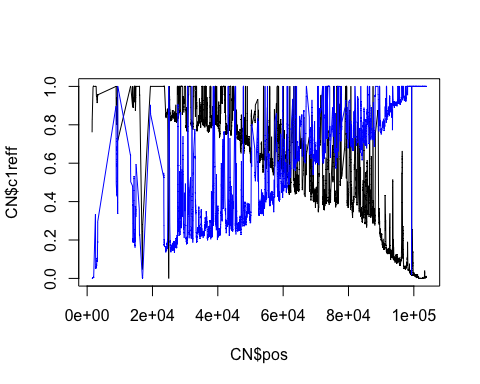
\includegraphics{BDMI_mapping_files/figure-latex/unnamed-chunk-23-1.pdf}

Plot mapped to cerevisiae. c1altf in black, c2altf in blue.
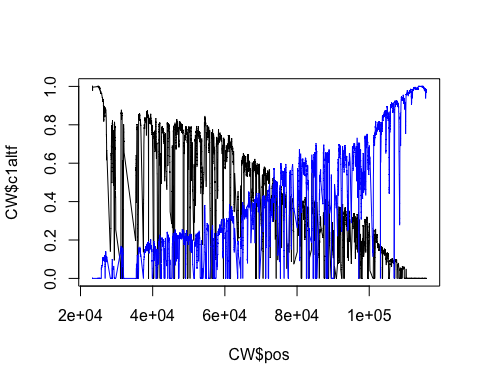
\includegraphics{BDMI_mapping_files/figure-latex/unnamed-chunk-24-1.pdf}

Cut SNPs with coverage 2 SD above mean.\\

\begin{Shaded}
\begin{Highlighting}[]
\FunctionTok{mean}\NormalTok{(CN}\SpecialCharTok{$}\NormalTok{c1cov)}
\end{Highlighting}
\end{Shaded}

\begin{verbatim}
## [1] 929.1932
\end{verbatim}

\begin{Shaded}
\begin{Highlighting}[]
\FunctionTok{sd}\NormalTok{(CN}\SpecialCharTok{$}\NormalTok{c1cov)}
\end{Highlighting}
\end{Shaded}

\begin{verbatim}
## [1] 242.5692
\end{verbatim}

\begin{Shaded}
\begin{Highlighting}[]
\NormalTok{cutCN1 }\OtherTok{\textless{}{-}} \FunctionTok{mean}\NormalTok{(CN}\SpecialCharTok{$}\NormalTok{c1cov)}\SpecialCharTok{+}\DecValTok{2}\SpecialCharTok{*}\FunctionTok{sd}\NormalTok{(CN}\SpecialCharTok{$}\NormalTok{c1cov)}

\FunctionTok{mean}\NormalTok{(CN}\SpecialCharTok{$}\NormalTok{c2cov)}
\end{Highlighting}
\end{Shaded}

\begin{verbatim}
## [1] 838.3074
\end{verbatim}

\begin{Shaded}
\begin{Highlighting}[]
\FunctionTok{sd}\NormalTok{(CN}\SpecialCharTok{$}\NormalTok{c2cov)}
\end{Highlighting}
\end{Shaded}

\begin{verbatim}
## [1] 199.0349
\end{verbatim}

\begin{Shaded}
\begin{Highlighting}[]
\NormalTok{cutCN2 }\OtherTok{\textless{}{-}} \FunctionTok{mean}\NormalTok{(CN}\SpecialCharTok{$}\NormalTok{c2cov)}\SpecialCharTok{+}\DecValTok{2}\SpecialCharTok{*}\FunctionTok{sd}\NormalTok{(CN}\SpecialCharTok{$}\NormalTok{c2cov)}

\FunctionTok{mean}\NormalTok{(CW}\SpecialCharTok{$}\NormalTok{c1cov)}
\end{Highlighting}
\end{Shaded}

\begin{verbatim}
## [1] 884.4712
\end{verbatim}

\begin{Shaded}
\begin{Highlighting}[]
\FunctionTok{sd}\NormalTok{(CW}\SpecialCharTok{$}\NormalTok{c1cov)}
\end{Highlighting}
\end{Shaded}

\begin{verbatim}
## [1] 230.6425
\end{verbatim}

\begin{Shaded}
\begin{Highlighting}[]
\NormalTok{cutCW1 }\OtherTok{\textless{}{-}} \FunctionTok{mean}\NormalTok{(CW}\SpecialCharTok{$}\NormalTok{c1cov)}\SpecialCharTok{+}\DecValTok{2}\SpecialCharTok{*}\FunctionTok{sd}\NormalTok{(CW}\SpecialCharTok{$}\NormalTok{c1cov)}

\FunctionTok{mean}\NormalTok{(CW}\SpecialCharTok{$}\NormalTok{c2cov)}
\end{Highlighting}
\end{Shaded}

\begin{verbatim}
## [1] 863.27
\end{verbatim}

\begin{Shaded}
\begin{Highlighting}[]
\FunctionTok{sd}\NormalTok{(CW}\SpecialCharTok{$}\NormalTok{c2cov)}
\end{Highlighting}
\end{Shaded}

\begin{verbatim}
## [1] 244.4764
\end{verbatim}

\begin{Shaded}
\begin{Highlighting}[]
\NormalTok{cutCW2 }\OtherTok{\textless{}{-}} \FunctionTok{mean}\NormalTok{(CW}\SpecialCharTok{$}\NormalTok{c2cov)}\SpecialCharTok{+}\DecValTok{2}\SpecialCharTok{*}\FunctionTok{sd}\NormalTok{(CW}\SpecialCharTok{$}\NormalTok{c2cov)}

\NormalTok{CNcut }\OtherTok{\textless{}{-}}\NormalTok{ CN[}\SpecialCharTok{{-}}\FunctionTok{which}\NormalTok{(CN}\SpecialCharTok{$}\NormalTok{c1cov }\SpecialCharTok{\textgreater{}}\NormalTok{ cutCN1 }\SpecialCharTok{|}\NormalTok{ CN}\SpecialCharTok{$}\NormalTok{c2cov }\SpecialCharTok{\textgreater{}}\NormalTok{ cutCN2),]}
\NormalTok{CWcut }\OtherTok{\textless{}{-}}\NormalTok{ CW[}\SpecialCharTok{!}\NormalTok{(CW}\SpecialCharTok{$}\NormalTok{c1cov }\SpecialCharTok{\textgreater{}}\NormalTok{ cutCW1 }\SpecialCharTok{|}\NormalTok{ CW}\SpecialCharTok{$}\NormalTok{c2cov }\SpecialCharTok{\textgreater{}}\NormalTok{ cutCW2),]}
\end{Highlighting}
\end{Shaded}

Plot the coverage of the original and versions with cutoff (cutoff in
red and purple).\\
Also add the cutoffs as lines.\\
Also add the frequencies (*1250 to fit on plot).

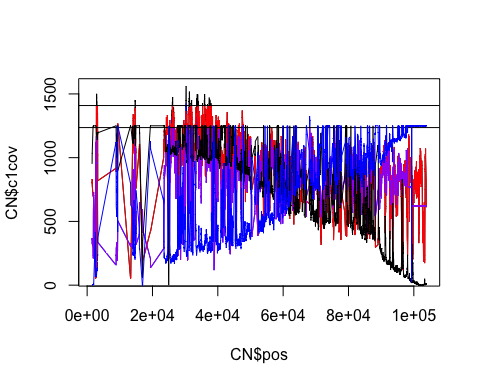
\includegraphics{BDMI_mapping_files/figure-latex/unnamed-chunk-26-1.pdf}
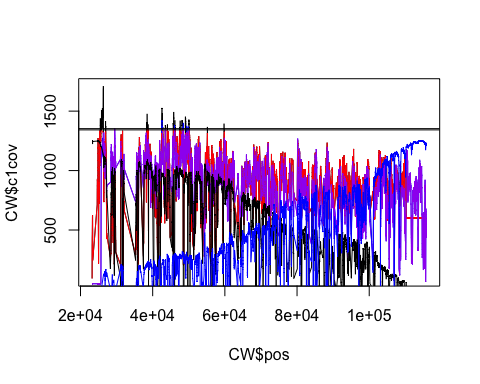
\includegraphics{BDMI_mapping_files/figure-latex/unnamed-chunk-26-2.pdf}
Still not good. Also, largish region with very few SNPs in paradoxus
mapping (and cer a bit).\\
\strut \\
Cut off bottom as well\\
Plot these in green and orange.

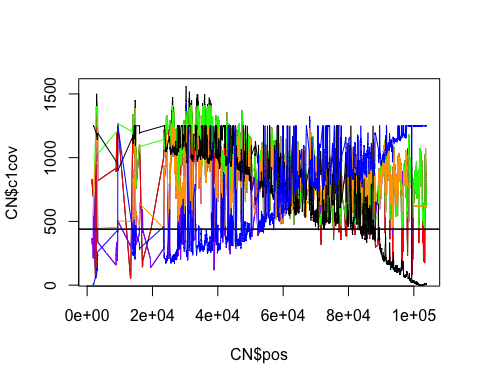
\includegraphics{BDMI_mapping_files/figure-latex/unnamed-chunk-27-1.pdf}
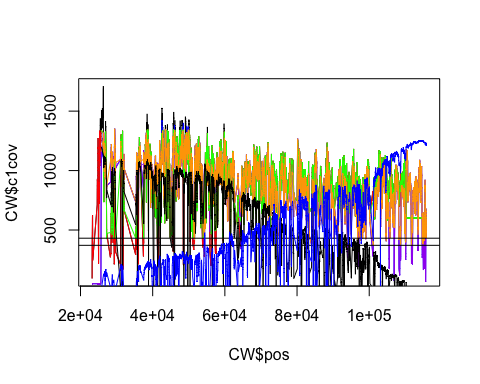
\includegraphics{BDMI_mapping_files/figure-latex/unnamed-chunk-27-2.pdf}
Got rid of some crazy peaks and smoothed it out a bit.\\
\strut \\
Now try requiring that called variants are variable in both samples
(within mapping to a single species).\\
This will cut off the ends, but we're not really interested in those.\\
Then plot again with original (lightest), cut2 (darker) and cut3
(darkest).

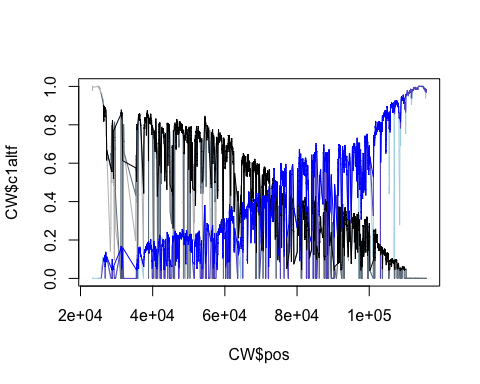
\includegraphics{BDMI_mapping_files/figure-latex/unnamed-chunk-28-1.pdf}
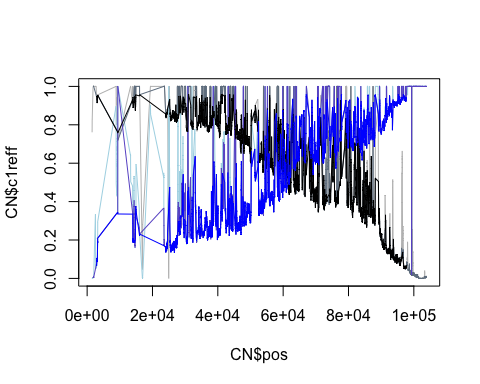
\includegraphics{BDMI_mapping_files/figure-latex/unnamed-chunk-28-2.pdf}
Still pretty crazy.\\
Tried requiring certain minimal minor allele frequency but doesn't seem
helpful, almost none with low cutoff.\\
\strut \\
Now will trim SNPs that are quite different from the median around them.
First, need to find out how big the region is.

\begin{verbatim}
## [1] 2837
\end{verbatim}

\begin{verbatim}
## [1] 97702
\end{verbatim}

\begin{verbatim}
## [1] 26354
\end{verbatim}

\begin{verbatim}
## [1] 110226
\end{verbatim}

Based on this, the region in paradoxus (N) is:\\
97702-2837=94865bp long\\
We expect the frequency to go from 0 to 1 in this region so, if went up
consistently, would change by 0.1 within:\\
94865/10=9486.5\\
so should be reasonable to expect that every SNP should be within 0.1 of
the median within \textasciitilde4743bp.\\
\strut \\
For cerevisiae (W): 110253-25752= 84501bp long\\
84501/10 = 8450.1\\
So will use 4225bp.\\
\strut \\
Also, do regions every 100bp. Plots the old frequencies from SNPs in
lighter colours and post-cut in darker colours. First, need to rename
columns.

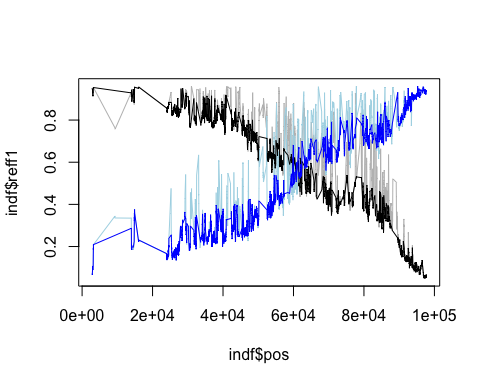
\includegraphics{BDMI_mapping_files/figure-latex/unnamed-chunk-30-1.pdf}
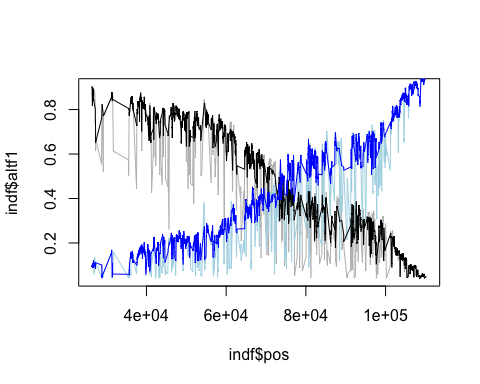
\includegraphics{BDMI_mapping_files/figure-latex/unnamed-chunk-30-2.pdf}
Find out how many cut:

\begin{Shaded}
\begin{Highlighting}[]
\FunctionTok{length}\NormalTok{(CNcut3}\SpecialCharTok{$}\NormalTok{chr)}
\end{Highlighting}
\end{Shaded}

\begin{verbatim}
## [1] 4670
\end{verbatim}

\begin{Shaded}
\begin{Highlighting}[]
\FunctionTok{length}\NormalTok{(CNcut4}\SpecialCharTok{$}\NormalTok{chr)}
\end{Highlighting}
\end{Shaded}

\begin{verbatim}
## [1] 3324
\end{verbatim}

\begin{Shaded}
\begin{Highlighting}[]
\FunctionTok{length}\NormalTok{(CWcut3}\SpecialCharTok{$}\NormalTok{chr)}
\end{Highlighting}
\end{Shaded}

\begin{verbatim}
## [1] 4713
\end{verbatim}

\begin{Shaded}
\begin{Highlighting}[]
\FunctionTok{length}\NormalTok{(CWcut4}\SpecialCharTok{$}\NormalTok{chr)}
\end{Highlighting}
\end{Shaded}

\begin{verbatim}
## [1] 3281
\end{verbatim}

Now plot with loess smoothing. Loess with span=0.25. Do for those mapped
to paradoxus first.
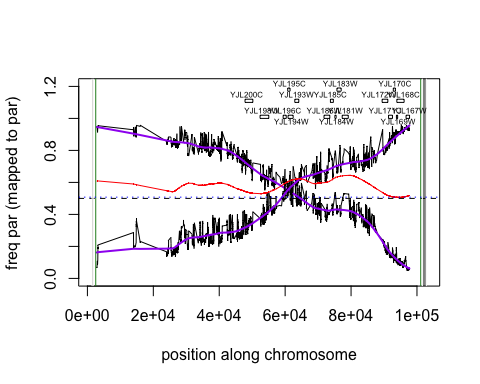
\includegraphics{BDMI_mapping_files/figure-latex/unnamed-chunk-32-1.pdf}
Plot for those mapped to paradoxus (N17) with loess smoothing.\\
Borders of original region in forestgreen. Rectangles where did
transformations.\\
Bottom 5\% of sum of fits in dotted blue line.\\
\strut \\
Now plot with loess smoothing. Loess with span=0.25. Do for those mapped
to cerevisiae.

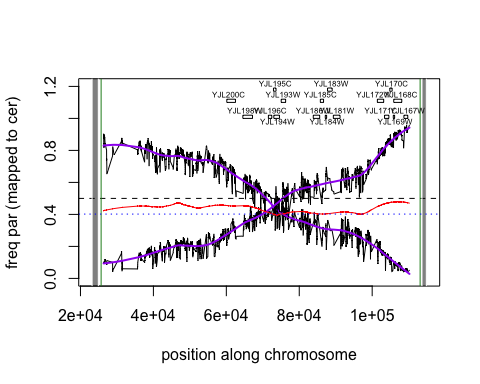
\includegraphics{BDMI_mapping_files/figure-latex/unnamed-chunk-33-1.pdf}
Plot for those mapped to cerevisiae (W303).\\
Borders of original region in forestgreen. Rectangles where did
transformations.\\
Bottom 5\% of sum of fits in dotted blue line.\\
\strut \\
Maybe could try taking an average of the two mappings??? But this would
also involve knowing which SNPs correspond.\\

\hypertarget{region-f}{%
\subsection{region F}\label{region-f}}

Do same as for region A and C. Only noted when something specific to
region F. Read in vcf files (mapped to N17 and W303).

Check that it worked.

\begin{Shaded}
\begin{Highlighting}[]
\FunctionTok{head}\NormalTok{(FN)}
\end{Highlighting}
\end{Shaded}

\begin{verbatim}
##           V1  V2 V3 V4 V5       V6   V7
## 1 N_17.chr15 473  .  A  C  9754.48 PASS
## 2 N_17.chr15 474  .  C  A  1821.05 PASS
## 3 N_17.chr15 488  .  A  C  2851.05 PASS
## 4 N_17.chr15 854  .  T  A 14780.50 PASS
## 5 N_17.chr15 862  .  A  T 16120.50 PASS
## 6 N_17.chr15 899  .  G  A 23453.50 PASS
##                                                                                                                                            V8
## 1       AC=3;AF=0.5;AN=6;BaseQRankSum=-3.2;DP=1039;FS=30.675;MLEAC=3;MLEAF=0.5;MQ=55.53;MQRankSum=1.8;QD=10.5;ReadPosRankSum=-4.019;SOR=0.079
## 2   AC=1;AF=0.167;AN=6;BaseQRankSum=0.635;DP=867;FS=18.713;MLEAC=1;MLEAF=0.167;MQ=50.1;MQRankSum=-9.369;QD=6.13;ReadPosRankSum=4.74;SOR=1.781
## 3 AC=1;AF=0.167;AN=6;BaseQRankSum=4.28;DP=804;FS=43.456;MLEAC=1;MLEAF=0.167;MQ=50.43;MQRankSum=-10.95;QD=10.92;ReadPosRankSum=-0.03;SOR=1.826
## 4     AC=3;AF=0.5;AN=6;BaseQRankSum=0.326;DP=2238;FS=12.83;MLEAC=3;MLEAF=0.5;MQ=58.48;MQRankSum=-8.245;QD=6.93;ReadPosRankSum=-1.59;SOR=1.013
## 5    AC=3;AF=0.5;AN=6;BaseQRankSum=-1.97;DP=2338;FS=10.742;MLEAC=3;MLEAF=0.5;MQ=58.3;MQRankSum=-8.842;QD=7.37;ReadPosRankSum=-2.342;SOR=0.937
## 6     AC=3;AF=0.5;AN=6;BaseQRankSum=-2.068;DP=2592;FS=5.925;MLEAC=3;MLEAF=0.5;MQ=57.86;MQRankSum=-11.36;QD=9.42;ReadPosRankSum=3.02;SOR=0.442
##               V9                                   V10
## 1 GT:AD:DP:GQ:PL   0/1/1:95,184:279:99:6859,264,0,3425
## 2 GT:AD:DP:GQ:PL  0/0/1:241,56:297:99:1828,0,557,10153
## 3 GT:AD:DP:GQ:PL   0/0/1:182,79:261:99:2858,0,310,7493
## 4 GT:AD:DP:GQ:PL 0/1/1:128,302:430:99:12184,525,0,4445
## 5 GT:AD:DP:GQ:PL 0/1/1:130,332:462:99:13157,608,0,4454
## 6 GT:AD:DP:GQ:PL 0/1/1:151,425:576:99:17503,825,0,5170
##                                        V11
## 1   0/0/1:545,105:650:99:2905,0,1322,22394
## 2         0/0/0:507,0:507:70:0,70,191,1800
## 3         0/0/0:507,0:507:70:0,70,191,1800
## 4 0/0/1:1566,138:1704:99:2606,0,4297,65260
## 5 0/0/1:1575,151:1726:99:2973,0,4282,65287
## 6 0/0/1:1691,224:1915:99:5960,0,4409,70421
\end{verbatim}

\begin{Shaded}
\begin{Highlighting}[]
\FunctionTok{head}\NormalTok{(FW)}
\end{Highlighting}
\end{Shaded}

\begin{verbatim}
##           V1    V2 V3 V4 V5      V6   V7
## 1 W303.chr15 17358  .  T  G 20422.3 PASS
## 2 W303.chr15 17384  .  T  C 31737.9 PASS
## 3 W303.chr15 17429  .  A  G 49415.5 PASS
## 4 W303.chr15 17448  .  C  T 49686.5 PASS
## 5 W303.chr15 17451  .  T  A 49790.5 PASS
## 6 W303.chr15 17472  .  A  G 50051.5 PASS
##                                                                                                                                       V8
## 1 AC=2;AF=0.333;AN=6;BaseQRankSum=-0.303;DP=2632;FS=16.717;MLEAC=2;MLEAF=0.333;MQ=60;MQRankSum=0;QD=28.36;ReadPosRankSum=-3.092;SOR=1.43
## 2  AC=2;AF=0.333;AN=6;BaseQRankSum=0.117;DP=2261;FS=16.873;MLEAC=2;MLEAF=0.333;MQ=60;MQRankSum=0;QD=28.73;ReadPosRankSum=0.389;SOR=0.941
## 3         AC=3;AF=0.5;AN=6;BaseQRankSum=1.09;DP=2897;FS=11.208;MLEAC=3;MLEAF=0.5;MQ=60;MQRankSum=0;QD=17.1;ReadPosRankSum=3.67;SOR=1.394
## 4        AC=3;AF=0.5;AN=6;BaseQRankSum=0.917;DP=2919;FS=5.331;MLEAC=3;MLEAF=0.5;MQ=60;MQRankSum=0;QD=17.02;ReadPosRankSum=4.01;SOR=1.076
## 5          AC=3;AF=0.5;AN=6;BaseQRankSum=5.22;DP=2936;FS=3.466;MLEAC=3;MLEAF=0.5;MQ=60;MQRankSum=0;QD=16.96;ReadPosRankSum=5.47;SOR=0.99
## 6         AC=3;AF=0.5;AN=6;BaseQRankSum=2.03;DP=3086;FS=6.236;MLEAC=3;MLEAF=0.5;MQ=60;MQRankSum=0;QD=16.22;ReadPosRankSum=1.72;SOR=1.086
##               V9                                    V10
## 1 GT:AD:DP:GQ:PL     0/0/0:1901,0:1901:0:0,0,3663,61661
## 2 GT:AD:DP:GQ:PL     0/0/0:1410,0:1410:70:0,70,191,1800
## 3 GT:AD:DP:GQ:PL 0/0/1:1582,82:1664:99:504,0,4514,67794
## 4 GT:AD:DP:GQ:PL 0/0/1:1586,84:1670:99:587,0,4521,68177
## 5 GT:AD:DP:GQ:PL 0/0/1:1601,85:1686:99:600,0,4563,68820
## 6 GT:AD:DP:GQ:PL 0/0/1:1732,83:1815:99:289,0,4964,74494
##                                        V11
## 1   0/1/1:108,612:720:99:20431,1511,0,2245
## 2    0/1/1:92,755:847:99:31750,1996,0,2218
## 3  0/1/1:83,1142:1225:99:48921,3187,0,1320
## 4 0/1/1:102,1147:1249:99:49109,3146,0,2084
## 5 0/1/1:101,1149:1250:99:49200,3155,0,2040
## 6 0/1/1:108,1163:1271:99:49772,3176,0,2297
\end{verbatim}

Rename the columns.\\
Cut down to the range for F:\\
range for F - YOL138C to YOL024W is region, did transformations YOL020W
to YOL141W for N17 - 272160 273938 to 46776 48863 for W303 - 288189
289967 to 58476 60563 Go a bit outside (1kb on either end).

Only keep the columns I want.\\

Plot outcome. Mapped to paradoxus, with f1reff in black, f2reff in blue.
\includegraphics{BDMI_mapping_files/figure-latex/unnamed-chunk-39-1.pdf}

Plot mapped to cerevisiae. f1altf in black, f2altf in blue.
\includegraphics{BDMI_mapping_files/figure-latex/unnamed-chunk-40-1.pdf}

Cut SNPs with coverage 2 SD above mean.\\

\begin{Shaded}
\begin{Highlighting}[]
\FunctionTok{mean}\NormalTok{(FN}\SpecialCharTok{$}\NormalTok{f1cov)}
\end{Highlighting}
\end{Shaded}

\begin{verbatim}
## [1] 754.733
\end{verbatim}

\begin{Shaded}
\begin{Highlighting}[]
\FunctionTok{sd}\NormalTok{(FN}\SpecialCharTok{$}\NormalTok{f1cov)}
\end{Highlighting}
\end{Shaded}

\begin{verbatim}
## [1] 212.1618
\end{verbatim}

\begin{Shaded}
\begin{Highlighting}[]
\NormalTok{cutFN1 }\OtherTok{\textless{}{-}} \FunctionTok{mean}\NormalTok{(FN}\SpecialCharTok{$}\NormalTok{f1cov)}\SpecialCharTok{+}\DecValTok{2}\SpecialCharTok{*}\FunctionTok{sd}\NormalTok{(FN}\SpecialCharTok{$}\NormalTok{f1cov)}

\FunctionTok{mean}\NormalTok{(FN}\SpecialCharTok{$}\NormalTok{f2cov)}
\end{Highlighting}
\end{Shaded}

\begin{verbatim}
## [1] 719.8816
\end{verbatim}

\begin{Shaded}
\begin{Highlighting}[]
\FunctionTok{sd}\NormalTok{(FN}\SpecialCharTok{$}\NormalTok{f2cov)}
\end{Highlighting}
\end{Shaded}

\begin{verbatim}
## [1] 255.309
\end{verbatim}

\begin{Shaded}
\begin{Highlighting}[]
\NormalTok{cutFN2 }\OtherTok{\textless{}{-}} \FunctionTok{mean}\NormalTok{(FN}\SpecialCharTok{$}\NormalTok{f2cov)}\SpecialCharTok{+}\DecValTok{2}\SpecialCharTok{*}\FunctionTok{sd}\NormalTok{(FN}\SpecialCharTok{$}\NormalTok{f2cov)}

\FunctionTok{mean}\NormalTok{(FW}\SpecialCharTok{$}\NormalTok{f1cov)}
\end{Highlighting}
\end{Shaded}

\begin{verbatim}
## [1] 805.2579
\end{verbatim}

\begin{Shaded}
\begin{Highlighting}[]
\FunctionTok{sd}\NormalTok{(FW}\SpecialCharTok{$}\NormalTok{f1cov)}
\end{Highlighting}
\end{Shaded}

\begin{verbatim}
## [1] 254.9876
\end{verbatim}

\begin{Shaded}
\begin{Highlighting}[]
\NormalTok{cutFW1 }\OtherTok{\textless{}{-}} \FunctionTok{mean}\NormalTok{(FW}\SpecialCharTok{$}\NormalTok{f1cov)}\SpecialCharTok{+}\DecValTok{2}\SpecialCharTok{*}\FunctionTok{sd}\NormalTok{(FW}\SpecialCharTok{$}\NormalTok{f1cov)}

\FunctionTok{mean}\NormalTok{(FW}\SpecialCharTok{$}\NormalTok{f2cov)}
\end{Highlighting}
\end{Shaded}

\begin{verbatim}
## [1] 693.7501
\end{verbatim}

\begin{Shaded}
\begin{Highlighting}[]
\FunctionTok{sd}\NormalTok{(FW}\SpecialCharTok{$}\NormalTok{f2cov)}
\end{Highlighting}
\end{Shaded}

\begin{verbatim}
## [1] 204.9185
\end{verbatim}

\begin{Shaded}
\begin{Highlighting}[]
\NormalTok{cutFW2 }\OtherTok{\textless{}{-}} \FunctionTok{mean}\NormalTok{(FW}\SpecialCharTok{$}\NormalTok{f2cov)}\SpecialCharTok{+}\DecValTok{2}\SpecialCharTok{*}\FunctionTok{sd}\NormalTok{(FW}\SpecialCharTok{$}\NormalTok{f2cov)}

\NormalTok{FNcut }\OtherTok{\textless{}{-}}\NormalTok{ FN[}\SpecialCharTok{{-}}\FunctionTok{which}\NormalTok{(FN}\SpecialCharTok{$}\NormalTok{f1cov }\SpecialCharTok{\textgreater{}}\NormalTok{ cutFN1 }\SpecialCharTok{|}\NormalTok{ FN}\SpecialCharTok{$}\NormalTok{f2cov }\SpecialCharTok{\textgreater{}}\NormalTok{ cutFN2),]}
\NormalTok{FWcut }\OtherTok{\textless{}{-}}\NormalTok{ FW[}\SpecialCharTok{!}\NormalTok{(FW}\SpecialCharTok{$}\NormalTok{f1cov }\SpecialCharTok{\textgreater{}}\NormalTok{ cutFW1 }\SpecialCharTok{|}\NormalTok{ FW}\SpecialCharTok{$}\NormalTok{f2cov }\SpecialCharTok{\textgreater{}}\NormalTok{ cutFW2),]}
\end{Highlighting}
\end{Shaded}

Plot the coverage of the original and versions with cutoff (cutoff in
red and purple).\\
Also add the cutoffs as lines.\\
Also add the frequencies (*1250 to fit on plot).

\includegraphics{BDMI_mapping_files/figure-latex/unnamed-chunk-42-1.pdf}
\includegraphics{BDMI_mapping_files/figure-latex/unnamed-chunk-42-2.pdf}
Still not good. Also, medium region with very few SNPs in cerevisiae
mapping.\\
\strut \\
Cut off bottom as well\\
Plot these in green and orange.
\includegraphics{BDMI_mapping_files/figure-latex/unnamed-chunk-43-1.pdf}
\includegraphics{BDMI_mapping_files/figure-latex/unnamed-chunk-43-2.pdf}
Got rid of some crazy peaks and smoothed it out a bit?\\
\strut \\
Now try requiring that called variants are variable in both samples
(within mapping to a single species).\\
This will cut off the ends, but we're not really interested in those.\\
Then plot again with original (lightest), cut2 (darker) and cut3
(darkest).

\includegraphics{BDMI_mapping_files/figure-latex/unnamed-chunk-44-1.pdf}
\includegraphics{BDMI_mapping_files/figure-latex/unnamed-chunk-44-2.pdf}
Still pretty crazy.\\
Now will trim SNPs that are quite different from the median around them.
First, need to find out how big the region is.

\begin{Shaded}
\begin{Highlighting}[]
\FunctionTok{min}\NormalTok{(FNcut3}\SpecialCharTok{$}\NormalTok{pos)}
\end{Highlighting}
\end{Shaded}

\begin{verbatim}
## [1] 51917
\end{verbatim}

\begin{Shaded}
\begin{Highlighting}[]
\FunctionTok{max}\NormalTok{(FNcut3}\SpecialCharTok{$}\NormalTok{pos)}
\end{Highlighting}
\end{Shaded}

\begin{verbatim}
## [1] 265747
\end{verbatim}

\begin{Shaded}
\begin{Highlighting}[]
\FunctionTok{min}\NormalTok{(FWcut3}\SpecialCharTok{$}\NormalTok{pos)}
\end{Highlighting}
\end{Shaded}

\begin{verbatim}
## [1] 66392
\end{verbatim}

\begin{Shaded}
\begin{Highlighting}[]
\FunctionTok{max}\NormalTok{(FWcut3}\SpecialCharTok{$}\NormalTok{pos)}
\end{Highlighting}
\end{Shaded}

\begin{verbatim}
## [1] 281704
\end{verbatim}

Based on this, the region in paradoxus (N) is:\\
265747-51917=213830bp long\\
We expect the frequency to go from 0 to 1 in this region so, if went up
consistently, would change by 0.1 within:\\
213830/10=21383\\
so should be reasonable to expect that every SNP should be within 0.1 of
the median within \textasciitilde10691bp.\\
\strut \\
For cerevisiae (W): 281704-66392= 215312bp long\\
215312/10 = 21531.2\\
So will use 10765bp.\\
\strut \\
Also, do regions every 100bp. Plots the old frequencies from SNPs in
lighter colours and post-cut in darker colours. First, need to rename
columns.

\includegraphics{BDMI_mapping_files/figure-latex/unnamed-chunk-46-1.pdf}
\includegraphics{BDMI_mapping_files/figure-latex/unnamed-chunk-46-2.pdf}

Find out how many cut:

\begin{Shaded}
\begin{Highlighting}[]
\FunctionTok{length}\NormalTok{(FNcut3}\SpecialCharTok{$}\NormalTok{chr)}
\end{Highlighting}
\end{Shaded}

\begin{verbatim}
## [1] 10588
\end{verbatim}

\begin{Shaded}
\begin{Highlighting}[]
\FunctionTok{length}\NormalTok{(FNcut4}\SpecialCharTok{$}\NormalTok{chr)}
\end{Highlighting}
\end{Shaded}

\begin{verbatim}
## [1] 7834
\end{verbatim}

\begin{Shaded}
\begin{Highlighting}[]
\FunctionTok{length}\NormalTok{(FWcut3}\SpecialCharTok{$}\NormalTok{chr)}
\end{Highlighting}
\end{Shaded}

\begin{verbatim}
## [1] 10534
\end{verbatim}

\begin{Shaded}
\begin{Highlighting}[]
\FunctionTok{length}\NormalTok{(FWcut4}\SpecialCharTok{$}\NormalTok{chr)}
\end{Highlighting}
\end{Shaded}

\begin{verbatim}
## [1] 7761
\end{verbatim}

Now plot with loess smoothing. Loess with span=0.25. Do for those mapped
to paradoxus first.
\includegraphics{BDMI_mapping_files/figure-latex/unnamed-chunk-48-1.pdf}

Plot for those mapped to paradoxus (N17) with loess smoothing.\\
Borders of original region in forestgreen. Rectangles where did
transformations.\\
Bottom 5\% of sum of fits in dotted blue line.\\
\strut \\
Now plot with loess smoothing. Loess with span=0.25. Do for those mapped
to cerevisiae.

\includegraphics{BDMI_mapping_files/figure-latex/unnamed-chunk-49-1.pdf}
Plot for those mapped to cerevisiae (W303).\\
Borders of original region in forestgreen. Rectangles where did
transformations.\\
Bottom 5\% of sum of fits in dotted blue line.\\
\strut \\
Next idea was to try and match up SNPs between the two mappings to only
keep those that correspond. This is not trivial, however, and I haven't
done that yet.\\

\hypertarget{region-e---try2}{%
\subsection{region E - try2}\label{region-e---try2}}

Do same. Read in vcf files (mapped to N17 and W303).

Check that it worked.

\begin{Shaded}
\begin{Highlighting}[]
\FunctionTok{head}\NormalTok{(E2N)}
\end{Highlighting}
\end{Shaded}

\begin{verbatim}
##           V1  V2 V3 V4 V5       V6   V7
## 1 N_17.chr15 473  .  A  C  5078.55 PASS
## 2 N_17.chr15 589  .  T  C  1050.10 PASS
## 3 N_17.chr15 607  .  C  A   696.05 PASS
## 4 N_17.chr15 621  .  T  G   476.05 PASS
## 5 N_17.chr15 854  .  T  A 10945.50 PASS
## 6 N_17.chr15 862  .  A  T 11244.50 PASS
##                                                                                                                                            V8
## 1  AC=3;AF=0.5;AN=6;BaseQRankSum=-2.779;DP=486;FS=19.281;MLEAC=3;MLEAF=0.5;MQ=55.98;MQRankSum=-5.233;QD=11.87;ReadPosRankSum=-3.689;SOR=0.168
## 2 AC=1;AF=0.167;AN=6;BaseQRankSum=-0.219;DP=599;FS=6.278;MLEAC=1;MLEAF=0.167;MQ=52.76;MQRankSum=-6.611;QD=6.4;ReadPosRankSum=-1.859;SOR=0.782
## 3 AC=1;AF=0.167;AN=6;BaseQRankSum=0.003;DP=517;FS=1.867;MLEAC=1;MLEAF=0.167;MQ=52.37;MQRankSum=-6.171;QD=4.67;ReadPosRankSum=-3.407;SOR=0.621
## 4     AC=1;AF=0.167;AN=6;BaseQRankSum=0.392;DP=479;FS=0;MLEAC=1;MLEAF=0.167;MQ=52.36;MQRankSum=-5.439;QD=3.63;ReadPosRankSum=-4.578;SOR=0.661
## 5  AC=3;AF=0.5;AN=6;BaseQRankSum=-3.001;DP=931;FS=25.681;MLEAC=3;MLEAF=0.5;MQ=57.59;MQRankSum=-8.876;QD=12.18;ReadPosRankSum=-1.463;SOR=1.539
## 6   AC=3;AF=0.5;AN=6;BaseQRankSum=-0.526;DP=960;FS=23.877;MLEAC=3;MLEAF=0.5;MQ=57.37;MQRankSum=-9.178;QD=12.25;ReadPosRankSum=-0.53;SOR=1.408
##               V9                                 V10
## 1 GT:AD:DP:GQ:PL     0/1/1:65,68:133:8:2400,8,0,2399
## 2 GT:AD:DP:GQ:PL 0/0/1:132,32:164:99:1055,0,301,5555
## 3 GT:AD:DP:GQ:PL  0/0/1:126,23:149:99:703,0,310,5338
## 4 GT:AD:DP:GQ:PL  0/0/1:114,17:131:99:483,0,292,4848
## 5 GT:AD:DP:GQ:PL 0/1/1:128,150:278:66:5815,66,0,4703
## 6 GT:AD:DP:GQ:PL 0/1/1:132,154:286:66:5906,66,0,4796
##                                     V11
## 1   0/0/1:212,83:295:99:2688,0,390,8651
## 2          0/0/0:379,0:379:0:0,0,0,6477
## 3      0/0/0:324,0:324:70:0,70,191,1800
## 4      0/0/0:328,0:328:70:0,70,191,1800
## 5 0/0/1:469,152:621:99:5140,0,952,19000
## 6 0/0/1:472,160:632:99:5348,0,936,19050
\end{verbatim}

\begin{Shaded}
\begin{Highlighting}[]
\FunctionTok{head}\NormalTok{(E2W)}
\end{Highlighting}
\end{Shaded}

\begin{verbatim}
##           V1    V2 V3 V4 V5     V6   V7
## 1 W303.chr15   340  .  G  C  35.06 PASS
## 2 W303.chr15   380  .  C  T 152.13 PASS
## 3 W303.chr15 13264  .  A  T  52.06 PASS
## 4 W303.chr15 14308  .  G  A  52.05 PASS
## 5 W303.chr15 14310  .  A  T  52.05 PASS
## 6 W303.chr15 14314  .  A  G  56.06 PASS
##                                                                                                                                            V8
## 1     AC=1;AF=0.167;AN=6;BaseQRankSum=-0.431;DP=79;FS=0;MLEAC=1;MLEAF=0.167;MQ=58.36;MQRankSum=-2.287;QD=3.51;ReadPosRankSum=-2.287;SOR=0.169
## 2 AC=1;AF=0.167;AN=6;BaseQRankSum=-2.996;DP=91;FS=1.719;MLEAC=1;MLEAF=0.167;MQ=54.95;MQRankSum=-4.218;QD=7.24;ReadPosRankSum=-0.818;SOR=0.368
## 3   AC=1;AF=0.167;AN=6;BaseQRankSum=0.826;DP=64;FS=2.881;MLEAC=1;MLEAF=0.167;MQ=42.96;MQRankSum=-1.025;QD=4.34;ReadPosRankSum=0.215;SOR=1.721
## 4                                                   AC=1;AF=0.167;AN=6;DP=71;FS=5.611;MLEAC=1;MLEAF=0.167;MQ=60;MQRankSum=0;QD=3.72;SOR=0.027
## 5          AC=1;AF=0.167;AN=6;BaseQRankSum=-2.211;DP=71;FS=5.611;MLEAC=1;MLEAF=0.167;MQ=60;MQRankSum=0;QD=3.72;ReadPosRankSum=0.183;SOR=0.027
## 6           AC=1;AF=0.167;AN=6;BaseQRankSum=-1.801;DP=69;FS=4.973;MLEAC=1;MLEAF=0.167;MQ=60;MQRankSum=0;QD=4.67;ReadPosRankSum=0.43;SOR=0.039
##               V9                            V10                          V11
## 1 GT:AD:DP:GQ:PL 0/0/0:67,0:67:70:0,70,191,1800  0/0/1:8,2:10:18:42,0,18,266
## 2 GT:AD:DP:GQ:PL 0/0/0:67,0:67:70:0,70,191,1800  0/0/1:12,9:21:9:159,0,9,361
## 3 GT:AD:DP:GQ:PL 0/0/0:52,0:52:70:0,70,191,1800 0/0/1:10,2:12:24:59,0,24,357
## 4 GT:AD:DP:GQ:PL 0/0/0:52,0:52:70:0,70,191,1800 0/0/1:12,2:14:30:59,0,30,509
## 5 GT:AD:DP:GQ:PL 0/0/0:52,0:52:70:0,70,191,1800 0/0/1:12,2:14:30:59,0,30,509
## 6 GT:AD:DP:GQ:PL 0/0/0:52,0:52:70:0,70,191,1800 0/0/1:10,2:12:24:63,0,24,423
\end{verbatim}

Rename the columns.\\
Cut down to the range for E:\\
range for E rep2 - YOL160W to YOL157C is region, did transformations
pau20 (YOL161C) to zps1 (YOL154W)\\
for N17 - 1590 2276 to 24900 25649\\
for W303 - 13641 14003 to 36750 37499\\
Go a bit outside (1kb on either end).

Only keep the columns I want.\\

Plot outcome. Mapped to paradoxus, with e21reff in black, e22reff in
blue.
\includegraphics{BDMI_mapping_files/figure-latex/unnamed-chunk-55-1.pdf}
Doesn't look great.\\

Plot mapped to cerevisiae. e21altf in black, e22altf in blue.
\includegraphics{BDMI_mapping_files/figure-latex/unnamed-chunk-56-1.pdf}
better???\\

Cut SNPs with coverage 2 SD above mean.\\

\begin{Shaded}
\begin{Highlighting}[]
\FunctionTok{mean}\NormalTok{(E2N}\SpecialCharTok{$}\NormalTok{e21cov)}
\end{Highlighting}
\end{Shaded}

\begin{verbatim}
## [1] 728.2364
\end{verbatim}

\begin{Shaded}
\begin{Highlighting}[]
\FunctionTok{sd}\NormalTok{(E2N}\SpecialCharTok{$}\NormalTok{e21cov)}
\end{Highlighting}
\end{Shaded}

\begin{verbatim}
## [1] 399.622
\end{verbatim}

\begin{Shaded}
\begin{Highlighting}[]
\NormalTok{cutE2N1 }\OtherTok{\textless{}{-}} \FunctionTok{mean}\NormalTok{(E2N}\SpecialCharTok{$}\NormalTok{e21cov)}\SpecialCharTok{+}\DecValTok{2}\SpecialCharTok{*}\FunctionTok{sd}\NormalTok{(E2N}\SpecialCharTok{$}\NormalTok{e21cov)}

\FunctionTok{mean}\NormalTok{(E2N}\SpecialCharTok{$}\NormalTok{e22cov)}
\end{Highlighting}
\end{Shaded}

\begin{verbatim}
## [1] 721.6316
\end{verbatim}

\begin{Shaded}
\begin{Highlighting}[]
\FunctionTok{sd}\NormalTok{(E2N}\SpecialCharTok{$}\NormalTok{e22cov)}
\end{Highlighting}
\end{Shaded}

\begin{verbatim}
## [1] 476.4803
\end{verbatim}

\begin{Shaded}
\begin{Highlighting}[]
\NormalTok{cutE2N2 }\OtherTok{\textless{}{-}} \FunctionTok{mean}\NormalTok{(E2N}\SpecialCharTok{$}\NormalTok{e22cov)}\SpecialCharTok{+}\DecValTok{2}\SpecialCharTok{*}\FunctionTok{sd}\NormalTok{(E2N}\SpecialCharTok{$}\NormalTok{e22cov)}

\FunctionTok{mean}\NormalTok{(E2W}\SpecialCharTok{$}\NormalTok{e21cov)}
\end{Highlighting}
\end{Shaded}

\begin{verbatim}
## [1] 525.7803
\end{verbatim}

\begin{Shaded}
\begin{Highlighting}[]
\FunctionTok{sd}\NormalTok{(E2W}\SpecialCharTok{$}\NormalTok{e21cov)}
\end{Highlighting}
\end{Shaded}

\begin{verbatim}
## [1] 202.9725
\end{verbatim}

\begin{Shaded}
\begin{Highlighting}[]
\NormalTok{cutE2W1 }\OtherTok{\textless{}{-}} \FunctionTok{mean}\NormalTok{(E2W}\SpecialCharTok{$}\NormalTok{e21cov)}\SpecialCharTok{+}\DecValTok{2}\SpecialCharTok{*}\FunctionTok{sd}\NormalTok{(E2W}\SpecialCharTok{$}\NormalTok{e21cov)}

\FunctionTok{mean}\NormalTok{(E2W}\SpecialCharTok{$}\NormalTok{e22cov)}
\end{Highlighting}
\end{Shaded}

\begin{verbatim}
## [1] 509.1424
\end{verbatim}

\begin{Shaded}
\begin{Highlighting}[]
\FunctionTok{sd}\NormalTok{(E2W}\SpecialCharTok{$}\NormalTok{e22cov)}
\end{Highlighting}
\end{Shaded}

\begin{verbatim}
## [1] 189.4075
\end{verbatim}

\begin{Shaded}
\begin{Highlighting}[]
\NormalTok{cutE2W2 }\OtherTok{\textless{}{-}} \FunctionTok{mean}\NormalTok{(E2W}\SpecialCharTok{$}\NormalTok{e22cov)}\SpecialCharTok{+}\DecValTok{2}\SpecialCharTok{*}\FunctionTok{sd}\NormalTok{(E2W}\SpecialCharTok{$}\NormalTok{e22cov)}

\NormalTok{E2Ncut }\OtherTok{\textless{}{-}}\NormalTok{ E2N[}\SpecialCharTok{{-}}\FunctionTok{which}\NormalTok{(E2N}\SpecialCharTok{$}\NormalTok{e21cov }\SpecialCharTok{\textgreater{}}\NormalTok{ cutE2N1 }\SpecialCharTok{|}\NormalTok{ E2N}\SpecialCharTok{$}\NormalTok{e22cov }\SpecialCharTok{\textgreater{}}\NormalTok{ cutE2N2),]}
\NormalTok{E2Wcut }\OtherTok{\textless{}{-}}\NormalTok{ E2W[}\SpecialCharTok{!}\NormalTok{(E2W}\SpecialCharTok{$}\NormalTok{e21cov }\SpecialCharTok{\textgreater{}}\NormalTok{ cutE2W1 }\SpecialCharTok{|}\NormalTok{ E2W}\SpecialCharTok{$}\NormalTok{e22cov }\SpecialCharTok{\textgreater{}}\NormalTok{ cutE2W2),]}
\end{Highlighting}
\end{Shaded}

Plot the coverage of the original and versions with cutoff (cutoff in
red and purple).\\
Also add the cutoffs as lines.\\
Also add the frequencies (*1250 to fit on plot).

\includegraphics{BDMI_mapping_files/figure-latex/unnamed-chunk-58-1.pdf}
\includegraphics{BDMI_mapping_files/figure-latex/unnamed-chunk-58-2.pdf}
Still not good.\\
\strut \\
Cut off bottom as well\\
Plot these in green and orange.
\includegraphics{BDMI_mapping_files/figure-latex/unnamed-chunk-59-1.pdf}
\includegraphics{BDMI_mapping_files/figure-latex/unnamed-chunk-59-2.pdf}
Now try requiring that called variants are variable in both samples
(within mapping to a single species).\\
This will cut off the ends, but we're not really interested in those.\\
Then plot again with original (lightest), cut2 (darker) and cut3
(darkest).

\includegraphics{BDMI_mapping_files/figure-latex/unnamed-chunk-60-1.pdf}
\includegraphics{BDMI_mapping_files/figure-latex/unnamed-chunk-60-2.pdf}
Still pretty crazy.\\
Now will trim SNPs that are quite different from the median around them.
First, need to find out how big the region is.

\begin{Shaded}
\begin{Highlighting}[]
\FunctionTok{min}\NormalTok{(E2Ncut3}\SpecialCharTok{$}\NormalTok{pos)}
\end{Highlighting}
\end{Shaded}

\begin{verbatim}
## [1] 854
\end{verbatim}

\begin{Shaded}
\begin{Highlighting}[]
\FunctionTok{max}\NormalTok{(E2Ncut3}\SpecialCharTok{$}\NormalTok{pos)}
\end{Highlighting}
\end{Shaded}

\begin{verbatim}
## [1] 22937
\end{verbatim}

\begin{Shaded}
\begin{Highlighting}[]
\FunctionTok{min}\NormalTok{(E2Wcut3}\SpecialCharTok{$}\NormalTok{pos)}
\end{Highlighting}
\end{Shaded}

\begin{verbatim}
## [1] 17358
\end{verbatim}

\begin{Shaded}
\begin{Highlighting}[]
\FunctionTok{max}\NormalTok{(E2Wcut3}\SpecialCharTok{$}\NormalTok{pos)}
\end{Highlighting}
\end{Shaded}

\begin{verbatim}
## [1] 34422
\end{verbatim}

Based on this, the region in paradoxus (N) is:\\
22937-854=22083bp long\\
We expect the frequency to go from 0 to 1 in this region so, if went up
consistently, would change by 0.1 within:\\
22083/10=2208.3\\
so should be reasonable to expect that every SNP should be within 0.1 of
the median within \textasciitilde1104bp.\\
\strut \\
For cerevisiae (W): 34422-17358= 17064bp long\\
17064/10 = 1706.4\\
So will use 853bp.\\
\strut \\
Also, do regions every 100bp. Plots the old frequencies from SNPs in
lighter colours and post-cut in darker colours. First, need to rename
columns.

\includegraphics{BDMI_mapping_files/figure-latex/unnamed-chunk-62-1.pdf}
\includegraphics{BDMI_mapping_files/figure-latex/unnamed-chunk-62-2.pdf}
Find out how many cut:

\begin{Shaded}
\begin{Highlighting}[]
\FunctionTok{length}\NormalTok{(E2Ncut3}\SpecialCharTok{$}\NormalTok{chr)}
\end{Highlighting}
\end{Shaded}

\begin{verbatim}
## [1] 609
\end{verbatim}

\begin{Shaded}
\begin{Highlighting}[]
\FunctionTok{length}\NormalTok{(E2Ncut4}\SpecialCharTok{$}\NormalTok{chr)}
\end{Highlighting}
\end{Shaded}

\begin{verbatim}
## [1] 329
\end{verbatim}

\begin{Shaded}
\begin{Highlighting}[]
\FunctionTok{length}\NormalTok{(E2Wcut3}\SpecialCharTok{$}\NormalTok{chr)}
\end{Highlighting}
\end{Shaded}

\begin{verbatim}
## [1] 442
\end{verbatim}

\begin{Shaded}
\begin{Highlighting}[]
\FunctionTok{length}\NormalTok{(E2Wcut4}\SpecialCharTok{$}\NormalTok{chr)}
\end{Highlighting}
\end{Shaded}

\begin{verbatim}
## [1] 303
\end{verbatim}

Now plot with loess smoothing. Loess with span=0.25. Do for those mapped
to paradoxus first. \#\#\#\#add genes\#\#\#\#
\includegraphics{BDMI_mapping_files/figure-latex/unnamed-chunk-64-1.pdf}
Not great but at least they cross?\\
Plot for those mapped to paradoxus (N17) with loess smoothing.\\
Borders of original region in forestgreen. Rectangles where did
transformations.\\
Bottom 5\% of sum of fits in dotted blue line.\\
\strut \\
Now plot with loess smoothing. Loess with span=0.25. Do for those mapped
to cerevisiae. \#\#\#add genes\#\#\#\#
\includegraphics{BDMI_mapping_files/figure-latex/unnamed-chunk-65-1.pdf}
Plot for those mapped to cerevisiae (W303).\\
Better? They cross\ldots.\\
Borders of original region in forestgreen. Rectangles where did
transformations.\\
Bottom 5\% of sum of fits in dotted blue line.\\
\strut \\
Next idea was to try and match up SNPs between the two mappings to only
keep those that correspond. This is not trivial, however, and I haven't
done that yet.\\

\end{document}
